\documentclass[10pt,compress]{beamer}

\usetheme{ohnosequences}
\usecolortheme{ohnosequences}
\usefonttheme{ohnosequences}
\usepackage{amssymb}
% \usepackage{unicode-math}
\usepackage{fontspec,xltxtra,xunicode}

\let\OldHref\href
\renewcommand{\href}[2]{\OldHref[pdfnewwindow]{#1}{{\textbf{#2}}}}

% \setbeamertemplate{caption}[numbered]
% \setbeamertemplate{caption label separator}{:}
% \setbeamercolor{caption name}{fg=normal text.fg}
% \usepackage{amssymb,amsmath}
% \usepackage{ifxetex,ifluatex}
% \usepackage{fixltx2e} % provides \textsubscript
% \usepackage{lmodern}
%
% \usepackage{fontspec,xltxtra,xunicode}
% \defaultfontfeatures{Mapping=tex-text}
\newcommand{\euro}{€}

% use upquote if available, for straight quotes in verbatim environments
\IfFileExists{upquote.sty}{\usepackage{upquote}}{}
% use microtype if available
% \IfFileExists{microtype.sty}{\usepackage{microtype}}{}

% verbatim and code highlighting: Solarized Light
\usepackage{color}
% SOLARIZED
\definecolor{solarized@base03}{HTML}{002B36}
\definecolor{solarized@base02}{HTML}{073642}
\definecolor{solarized@base01}{HTML}{586e75}
\definecolor{solarized@base00}{HTML}{657b83}
\definecolor{solarized@base0}{HTML}{839496}
\definecolor{solarized@base1}{HTML}{93a1a1}
\definecolor{solarized@base2}{HTML}{EEE8D5}
\definecolor{solarized@base3}{HTML}{FDF6E3}
\definecolor{solarized@yellow}{HTML}{B58900}
\definecolor{solarized@orange}{HTML}{CB4B16}
\definecolor{solarized@red}{HTML}{DC322F}
\definecolor{solarized@magenta}{HTML}{D33682}
\definecolor{solarized@violet}{HTML}{6C71C4}
\definecolor{solarized@blue}{HTML}{268BD2}
\definecolor{solarized@cyan}{HTML}{2AA198}
\definecolor{solarized@green}{HTML}{859900}

\usepackage{fancyvrb}
\newcommand{\VerbBar}{|}
\newcommand{\VERB}{\Verb[commandchars=\\\{\}]}
\DefineVerbatimEnvironment{Highlighting}{Verbatim}{fontsize=\footnotesize,commandchars=\\\{\}}

% Add ',fontsize=\small' for more characters per line
\usepackage{framed}
% this is solarized light
\definecolor{shadecolor}{RGB}{253,246,227} % solarized@base3
\newenvironment{Shaded}{\vspace{\baselineskip}\begin{shaded}}{\end{shaded}\vspace{\baselineskip}}
% colored backgrd for verb
\let\oldverbatim=\verbatim
\let\endoldverbatim=\endverbatim
  \vspace{\baselineskip}
\renewenvironment{verbatim}[1]{%
  \scriptsize
  \par\setstretch{1}
  \begin{shaded}
  \begin{oldverbatim}{#1}%
}%
{%
  \end{oldverbatim}%
  \end{shaded}
  \vspace{\baselineskip}
}

\newcommand{\KeywordTok}[1]{\textcolor{solarized@base00}{\textbf{#1}}}
\newcommand{\DataTypeTok}[1]{\textcolor{solarized@blue}{#1}}
\newcommand{\DecValTok}[1]{\textcolor{solarized@violet}{#1}}
\newcommand{\BaseNTok}[1]{\textcolor{solarized@violet}{#1}}
\newcommand{\FloatTok}[1]{\textcolor{solarized@violet}{#1}}
\newcommand{\CharTok}[1]{\textcolor{solarized@cyan}{#1}}
\newcommand{\StringTok}[1]{\textcolor{solarized@violet}{#1}}
\newcommand{\CommentTok}[1]{\textcolor{solarized@base1}{\textit{#1}}}
\newcommand{\OtherTok}[1]{\textcolor{solarized@green}{#1}}
\newcommand{\AlertTok}[1]{\textcolor{solarized@yellow}{\textbf{#1}}}
% In Scala: method calls
\newcommand{\FunctionTok}[1]{\textcolor{solarized@base1}{#1}}
\newcommand{\RegionMarkerTok}[1]{\textcolor{solarized@base1}{#1}}
\newcommand{\ErrorTok}[1]{\textcolor{solarized@red}{\textbf{#1}}}
\newcommand{\NormalTok}[1]{\textcolor{solarized@base00}{#1}}


% allow to break lines more easily on tt text
% http://tex.stackexchange.com/questions/52850/temporarily-increase-the-limit-on-space-size
\let\OldTexttt\texttt
\renewcommand{\texttt}[1]{ \emergencystretch=2em \OldTexttt{#1} }
% maybe?
\setlength{\emergencystretch}{3em}  % prevent overfull lines

\usepackage{graphicx}
\makeatletter
\def\maxwidth{\ifdim\Gin@nat@width>\linewidth\linewidth\else\Gin@nat@width\fi}
\def\maxheight{\ifdim\Gin@nat@height>\textheight0.8\textheight\else\Gin@nat@height\fi}
\makeatother
% Scale images if necessary, so that they will not overflow the page
% margins by default, and it is still possible to overwrite the defaults
% using explicit options in \includegraphics[width, height, ...]{}
\setkeys{Gin}{width=\maxwidth,height=\maxheight,keepaspectratio}

% Comment these out if you don't want a slide with just the
% part/section/subsection/subsubsection title:
% \AtBeginPart{
%   \let\insertpartnumber\relax
%   \let\partname\relax
%   \frame{\partpage}
% }
% \AtBeginSection{
%   \let\insertsectionnumber\relax
%   \let\sectionname\relax
%   \frame{\sectionpage}
% }
% \AtBeginSubsection{
%   \let\insertsubsectionnumber\relax
%   \let\subsectionname\relax
%   \frame{\subsectionpage}
% }

\usepackage[normalem]{ulem}
% avoid problems with \sout in headers with hyperref:
\pdfstringdefDisableCommands{\renewcommand{\sout}{}}
% \setlength{\parindent}{0pt}
% \setlength{\parskip}{6pt plus 2pt minus 1pt}
% \setlength{\emergencystretch}{3em}  % prevent overfull lines
% \providecommand{\tightlist}{%
%   \setlength{\itemsep}{0pt}\setlength{\parskip}{0pt}}
% % \setcounter{secnumdepth}{0}
% 
\hypersetup{
  setpagesize=false, % page size defined by xetex
  unicode=false, % unicode breaks when used with xetex
  xetex,
  pdfnewwindow,
  colorlinks,%
  citecolor=OldCyan-Dark,%
  filecolor=OldCyan-Dark,%
  linkcolor=OldCyan-Dark,%
  urlcolor=OldCyan-Dark,
  urlbordercolor=OldCyan-Dark
}



\usepackage{booktabs}
\usepackage[scale=2]{ccicons}

\title{Slides with Pandoc}
\subtitle{an introduction}
\author{Eduardo Pareja-Tobes}
\date{14 March 2023}

\institute{
  \href{http://era7bioinformatics.com}{{Era7} {\color{Grey-Light}bioinformatics}} - {\color{Salmon-Dark}oh}{\color{LightAmber-Dark}no}{\color{Grey}sequences}{\color{Salmon-Dark}!}
}

\begin{document}
\maketitle


% 
\section{The idea}\label{the-idea}

\begin{frame}{what?}

\begin{block}{markdown sources}

You write your \emph{slides} using \textbf{Markdown}, working with them
as you would with any markdown file; you can use all your favorite
\texttt{pandoc} features too!

\end{block}

\begin{block}{PDF slides}

Then, \texttt{pandoc} and \texttt{XeTeX} will convert your source to
\texttt{pdf} using a custom \texttt{beamer} template. That sounds
involved, but is already automated for you.

\end{block}

\end{frame}

\section{How}\label{how}

\begin{frame}[fragile]{Making slides}

Use level \emph{one} headings to make \emph{sections}, and level
\emph{two} headings for \emph{slides}. You can introduce a new slide at
any point with \emph{4} or more dashes \texttt{-\/-\/-\/-}. This is
sometimes handy for displaying images or a lot of code.

\begin{Shaded}
\begin{Highlighting}[]
\FunctionTok{# A section}

\FunctionTok{## Now a slide}

\NormalTok{Hola!}

\NormalTok{----}

\NormalTok{Another slide here!}
\end{Highlighting}
\end{Shaded}

\end{frame}

\section{Formatting}\label{formatting}

\begin{frame}{Standard Markdown}

Everything works the same as for any markdown document. You have
\textbf{bold}, \emph{italic} and \emph{\textbf{bold italic}} text;
\sout{strikeout}, \href{http://ohnosequences.com}{links} and of course
$\lim_{n \to \infty} B(n) = c$. Block quotes work too:

\begin{quote}
quotations are a byproduct of impermanence

\textbf{Someone}, 2018
\end{quote}

\begin{enumerate}
\def\labelenumi{\arabic{enumi}.}
\itemsep1pt\parskip0pt\parsep0pt
\item
  and also lists
\item
  numbered or not, nested, \ldots{}

  \begin{itemize}
  \itemsep1pt\parskip0pt\parsep0pt
  \item
    the order is sometimes
  \item
    not so important
  \end{itemize}
\end{enumerate}

\end{frame}

\begin{frame}{Images}

\begin{figure}[htbp]
\centering
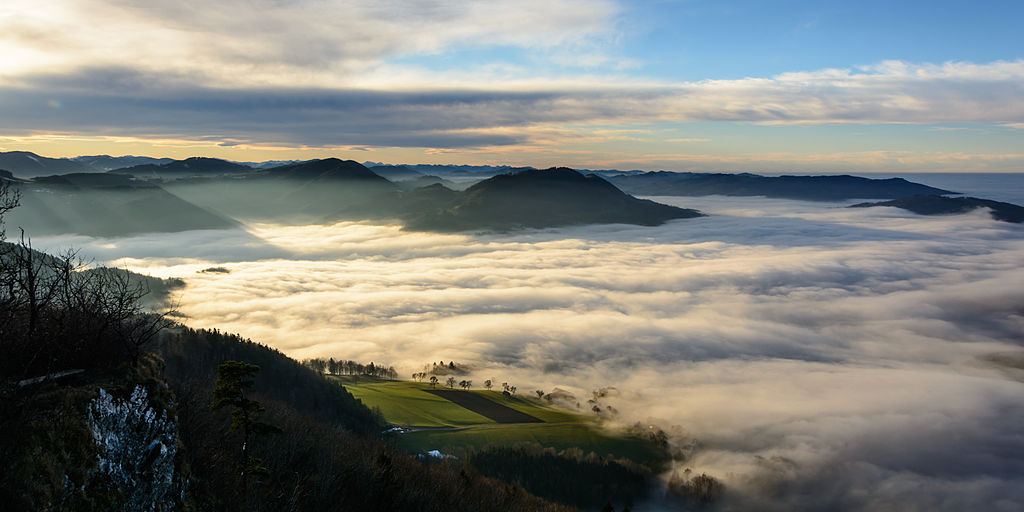
\includegraphics{images/valley.jpg}
\caption{A nice valley}
\end{figure}

\end{frame}

\begin{frame}{Images}

\begin{figure}[htbp]
\centering
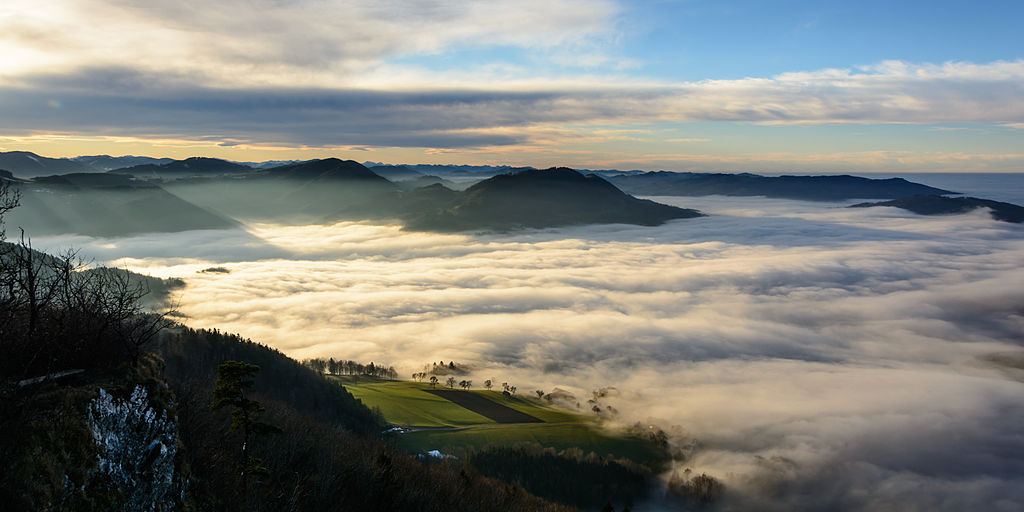
\includegraphics{images/valley.jpg}
\end{figure}

\end{frame}

\begin{frame}

\begin{figure}[htbp]
\centering
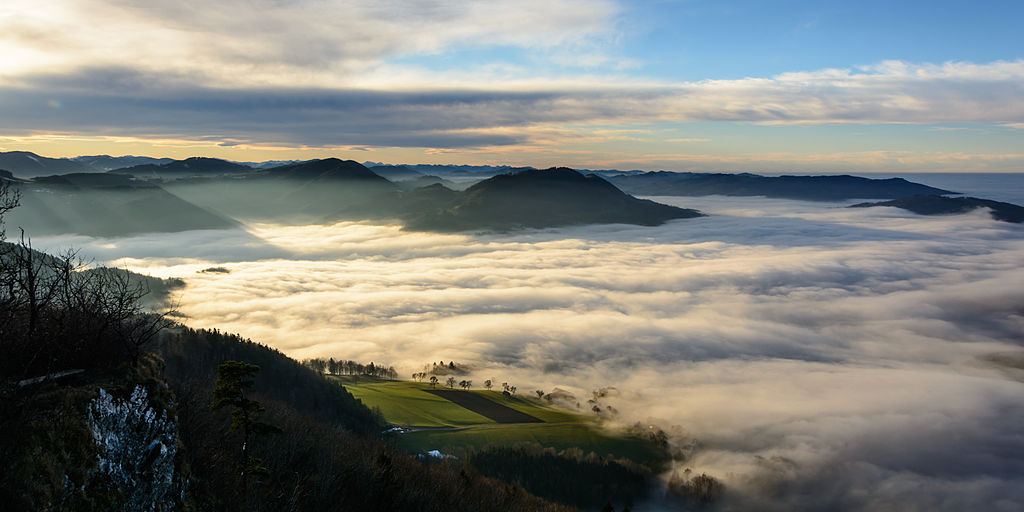
\includegraphics{images/valley.jpg}
\caption{A nice valley again}
\end{figure}

\end{frame}

\begin{frame}[fragile]{Code highlighting}

Works reasonably well. The awful Haskell syntax in all its glory:

\begin{Shaded}
\begin{Highlighting}[]
\KeywordTok{data} \DataTypeTok{DList} \NormalTok{a }\FunctionTok{=} \DataTypeTok{DLNode} \NormalTok{(}\DataTypeTok{DList} \NormalTok{a) a (}\DataTypeTok{DList} \NormalTok{a)}

\OtherTok{takeF ::} \DataTypeTok{Integer} \OtherTok{->} \DataTypeTok{DList} \NormalTok{a }\OtherTok{->} \NormalTok{[a]}
\NormalTok{takeF }\DecValTok{0}     \NormalTok{_                   }\FunctionTok{=} \NormalTok{[]}
\NormalTok{takeF (n }\FunctionTok{+} \DecValTok{1}\NormalTok{) (}\DataTypeTok{DLNode} \NormalTok{_ x next) }\FunctionTok{=} \NormalTok{x }\FunctionTok{:} \NormalTok{(takeF n next)}

\OtherTok{takeR ::} \DataTypeTok{Show} \NormalTok{a }\OtherTok{=>} \DataTypeTok{Integer} \OtherTok{->} \DataTypeTok{DList} \NormalTok{a }\OtherTok{->} \NormalTok{[a]}
\NormalTok{takeR }\DecValTok{0}     \NormalTok{_                   }\FunctionTok{=} \NormalTok{[]}
\NormalTok{takeR (n }\FunctionTok{+} \DecValTok{1}\NormalTok{) (}\DataTypeTok{DLNode} \NormalTok{prev x _) }\FunctionTok{=} \NormalTok{x }\FunctionTok{:} \NormalTok{(takeR n prev)}
\end{Highlighting}
\end{Shaded}

\end{frame}

\begin{frame}{Code highlighting}

Sadly, the Scala syntax definition that Pandoc uses is awful. See
\href{https://github.com/jgm/highlighting-kate/issues/71}{jgm/highlighting-kate\#71}

``` scala // Scala looks awful! case class test(val x: Boolean) \{

lazy val x = 2 type T = Int def oh: String = ``Buh!'' \} ```

\end{frame}

\section{Slides specific bits}\label{slides-specific-bits}

\begin{frame}{Basic animations}

\begin{block}{Incremental lists}

Sometimes we want to display items from a list incrementally:

\begin{itemize}[<+->]
\itemsep1pt\parskip0pt\parsep0pt
\item
  first this,
\item
  then that
\item
  and also this too
\end{itemize}

Can be a nice touch sometimes; do not abuse it though.

\end{block}

\end{frame}

\begin{frame}{Basic animations}

\begin{block}{Pauses}

Pause is a bit misleading here. The effect is that a slide displays at
first only part of your text.

\pause

Once you advance to the next, you get the same as before plus some added
content. It can be a nice addition if you remember \emph{where} those
pauses are.

\pause

It can also be a bit

\pause

tiring.

\end{block}

\end{frame}

\section{Questions?}\label{questions}

\end{document}
